\section{Preliminaries}







\subsection{Problem Setup}


Given samples, $x = (x_j)_{j=1}^s \in \RR^s$ and labels $y = (y_j)_{j=1}^s \in \RR^s$, we consider the following least squares approximation problem:

\begin{equation}\label{eq:leastsquares}
\begin{aligned}
    &\min_{\bm \xi} L(\bm \xi) =  \frac{1}{2} \sum_{j=1}^s |f_{\bm \xi}(x_j) - y_j|^2,\\
    &\mbox{ where } \,\,\, f_{\bm \xi}(x) = \sum_{i=1}^m \epsilon_i \langle (x, 1), (u_i, v_i) \rangle_+, \quad \bm \xi = (\bm \epsilon \in \{-1, 0, 1\}^m, \bm u \in \RR^m, \bm v \in \RR^m),
\end{aligned}
\end{equation}

where $\langle \cdot, \cdot \rangle_+$ is the ReLU operator. Our functional space $\mathcal F_m = \{f_{\bm \xi}: \RR\rightarrow \RR, \, \,\textbf{} {\bm \theta} \in \RR^{3m}\}$ is the family of 1D feedforward shallow ReLU networks with exactly $m$ neurons $(\epsilon_i, u_i, v_i)$. It is easy to see that $\mathcal F_m$ is contained in the the set $CPL_m$ of \emph{continuous piecewise-linear} functions with at most $m$ knots. The knots of $f_{\bm \xi}$ are the points where the operand inside a ReLU activation changes sign:

\begin{equation}\label{eq:knots}
e_i = -\frac{u_i}{v_i}, \quad u_i \ne 0, \quad i=1,\ldots,m.
\end{equation}

Written this way, we can easily visualize a feedforward network and its knots (see Figure~\ref{fig:knots}). In this paper, we focus on the overparameterized setting $m \gg s$. In particular, many parameter values can interpolate the samples and have zero loss $L(\bm \xi) = 0$.

\begin{remark}
The definition \eqref{eq:leastsquares} is slightly different than traditional neural network parameterization. Note however, that due to homogeneity these two are equivalent. We chose this parameterization because it makes our proofs clearer and it is very easy to visualize.
\end{remark}

\begin{figure}
    \centering
    \minipage{0.5\textwidth}
    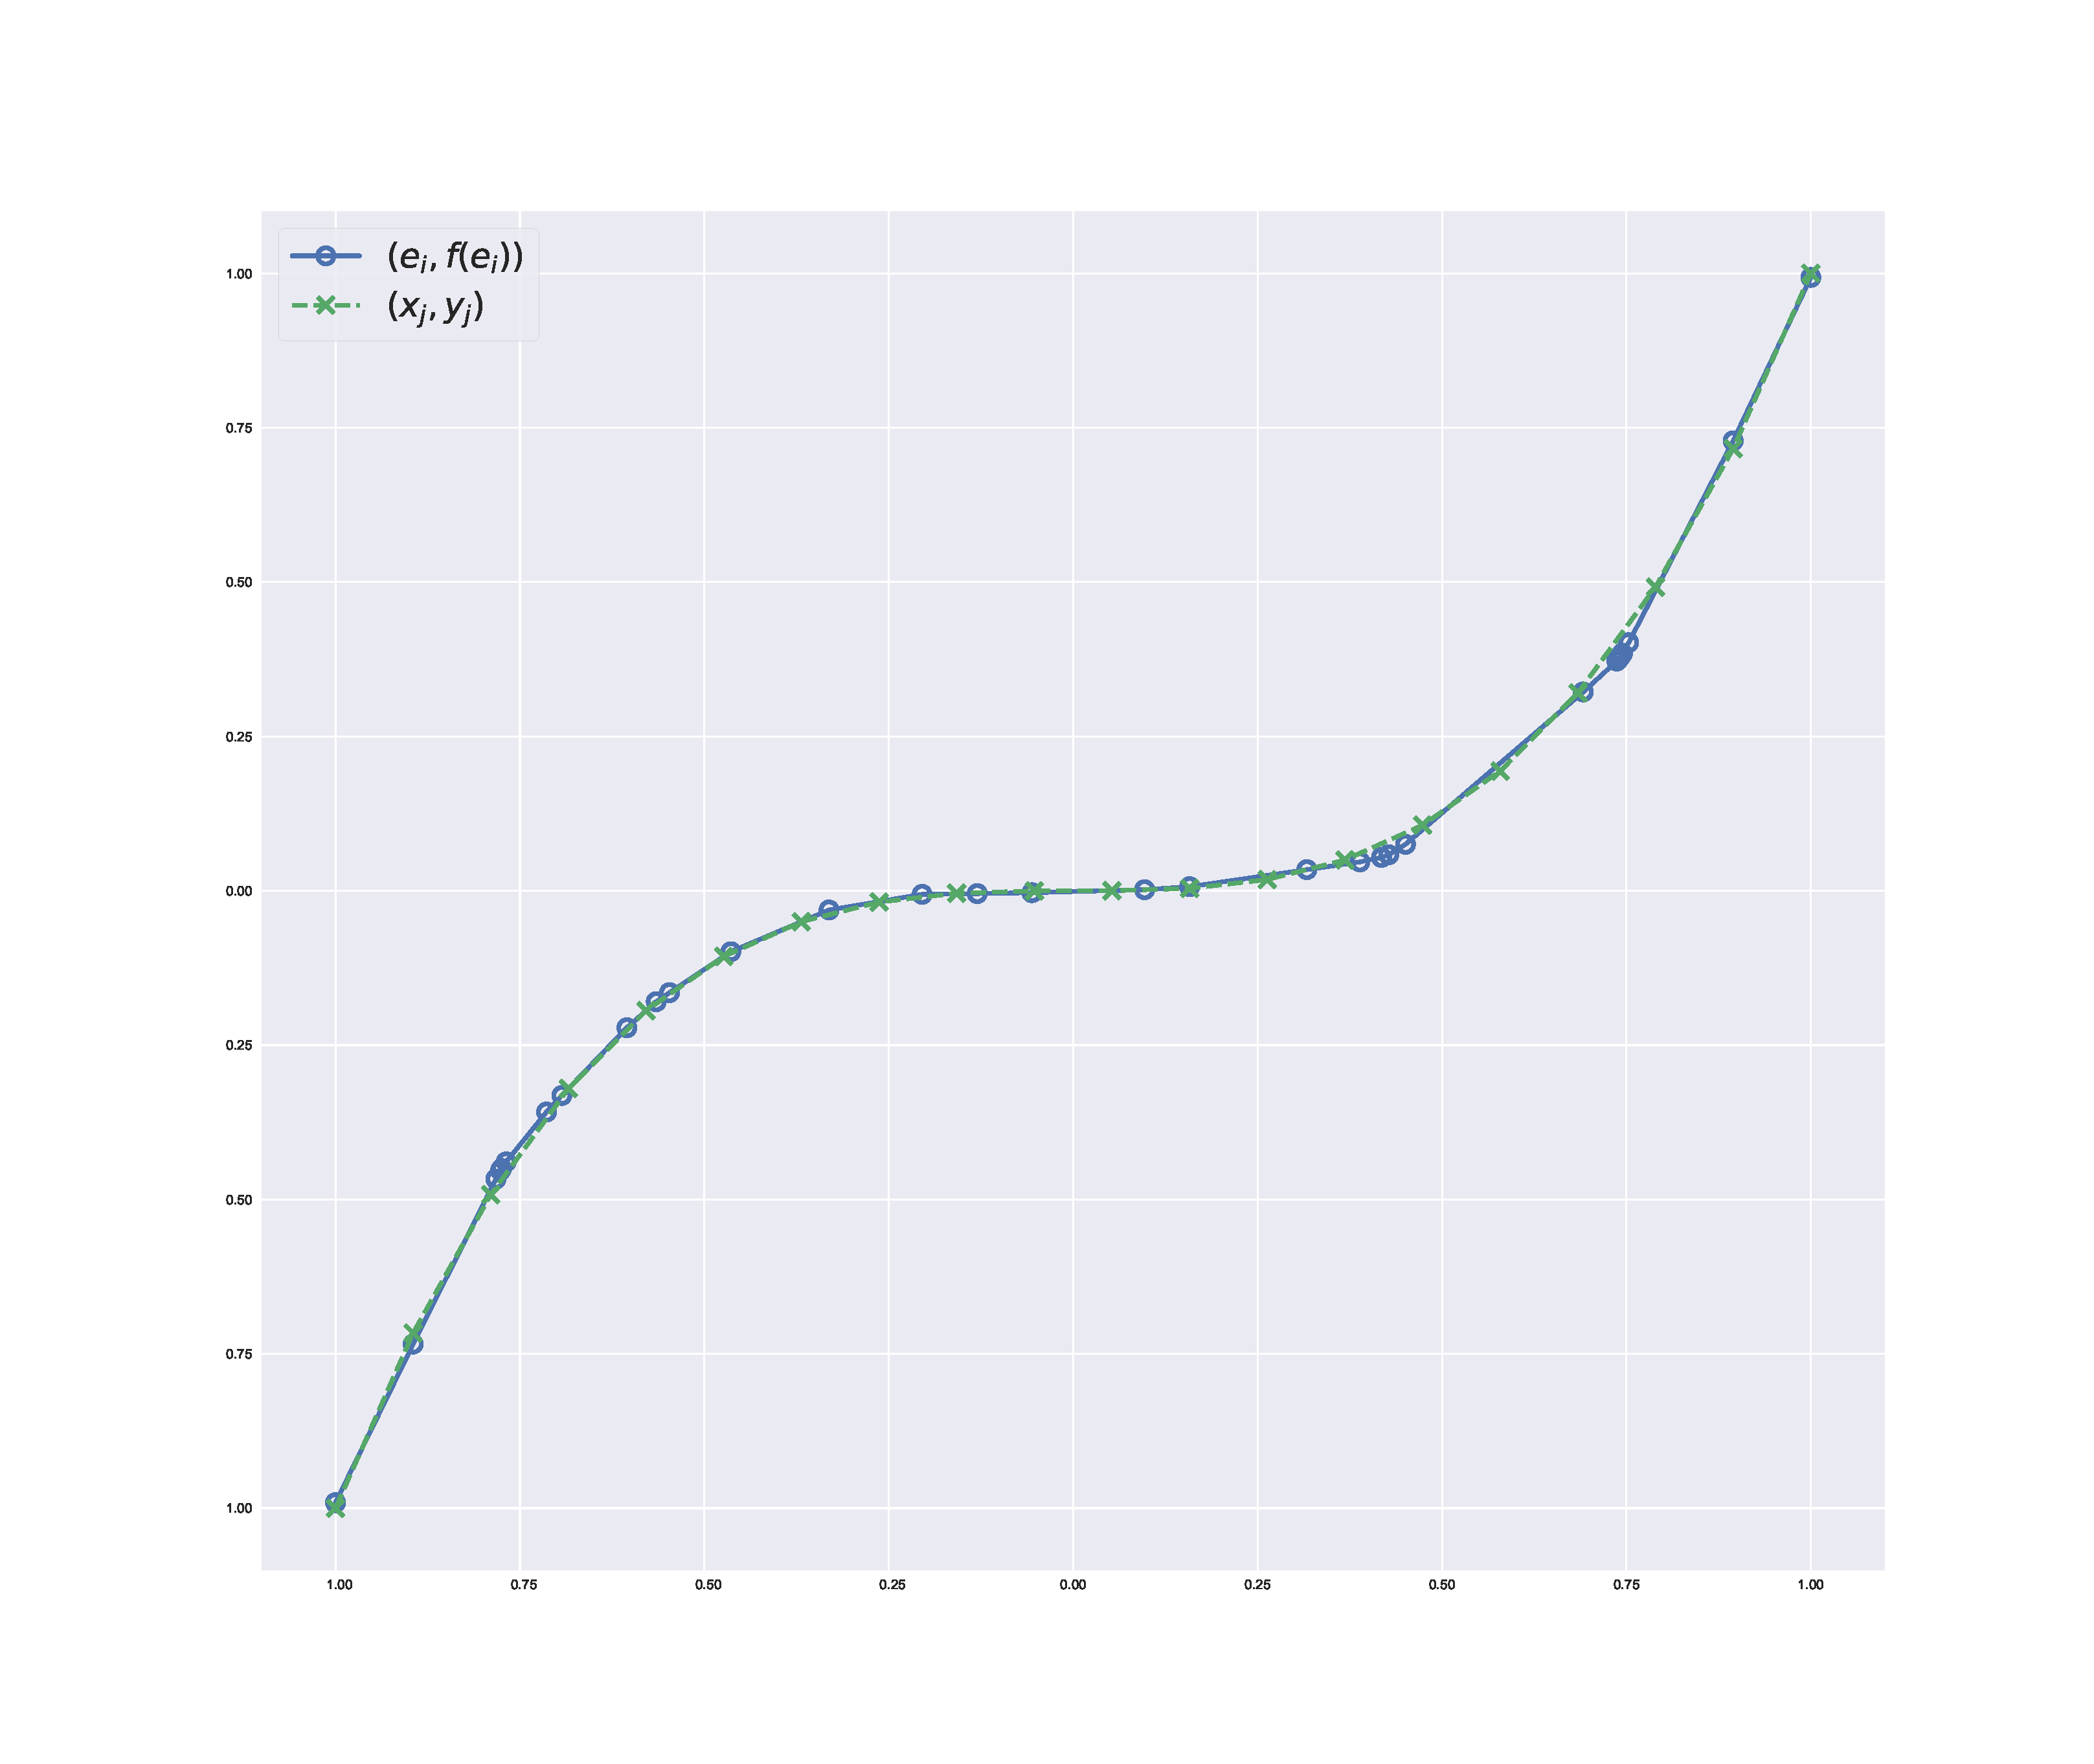
\includegraphics[width=\textwidth]{figures/knots2.pdf}
    \endminipage\hfill
    \minipage{0.5\textwidth}
    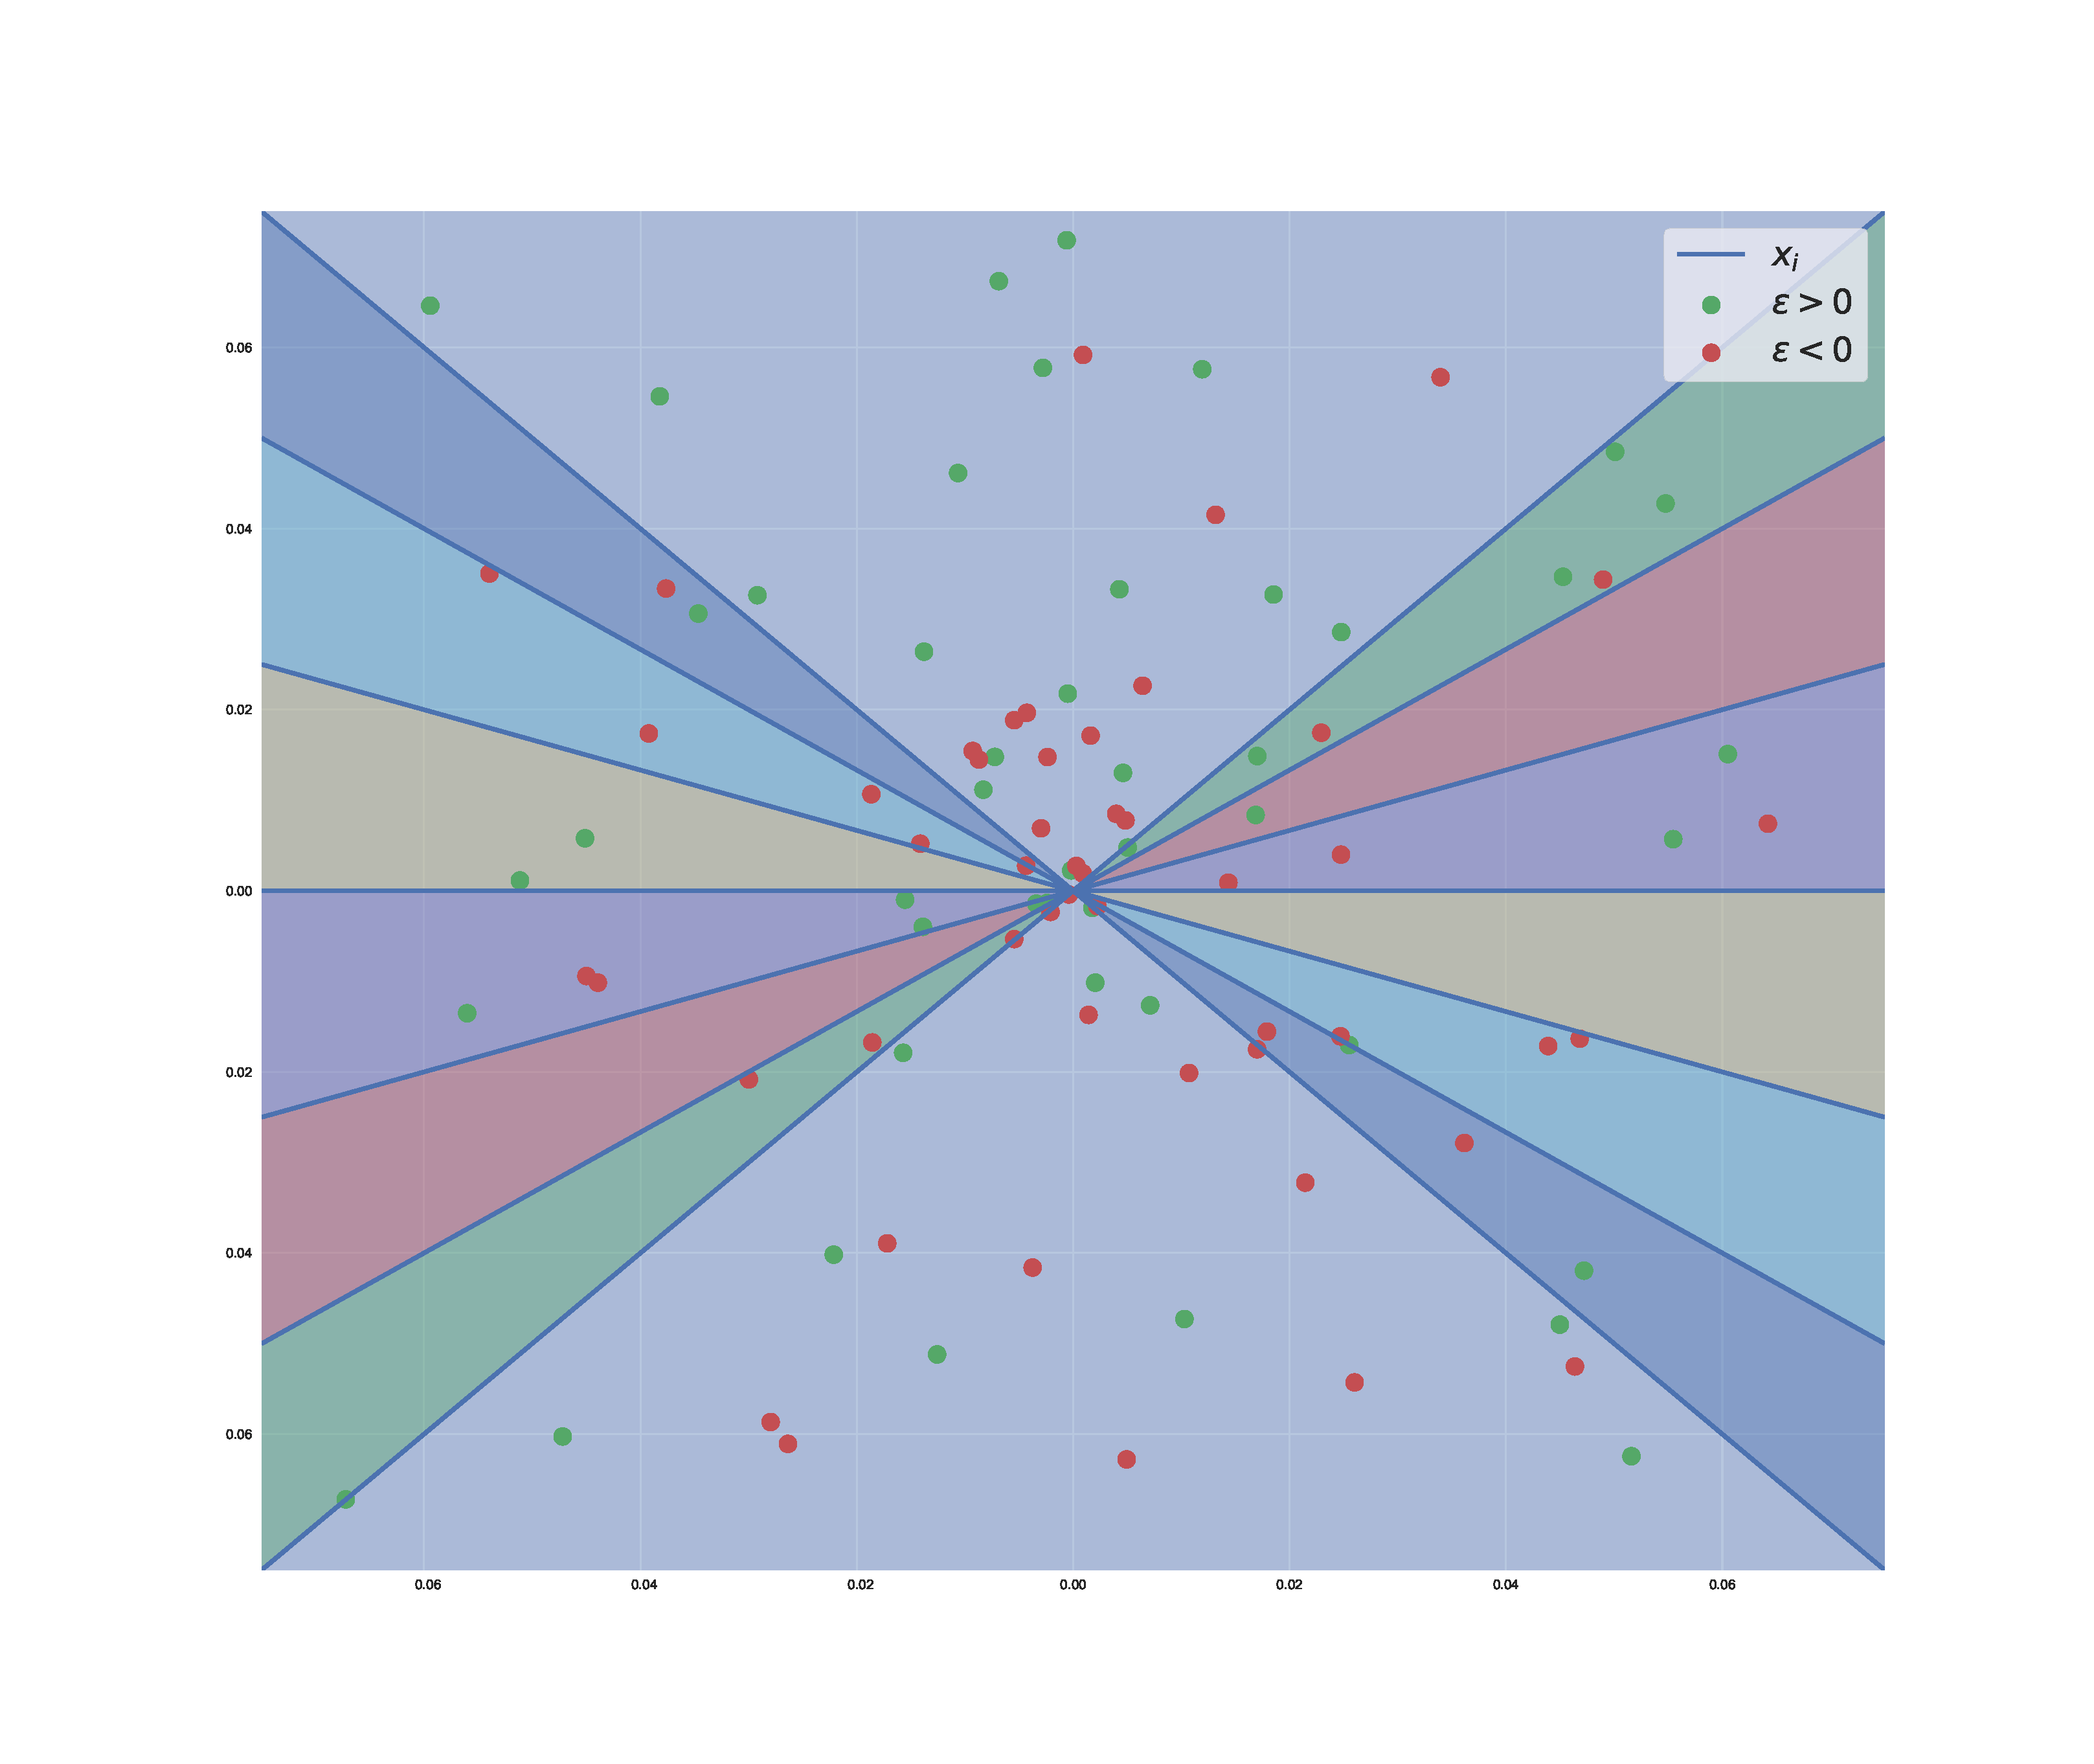
\includegraphics[width=\textwidth]{figures/phaseplot_eg.pdf}
    \endminipage\hfill
    
    
    \caption{\textit{Left:} input samples $(x, y) = (x_j, y_j)_{j=1}^s$ (blue x's) to which we fit a neural network $f_{\bm \xi}(x)$ using the least squares loss \eqref{eq:leastsquares}. $f_{\bm \xi}(x)$ is piecewise linear with the boundaries between pieces occurring at $(e_i, f_{\bm \xi}(e_i))_{i=1}^m$ (green circles). These points correspond to when the operand to one of the ReLUs in \eqref{eq:leastsquares} goes from positive to negative or vice-versa. \textit{Right:} the neurons $\xi_i = (\epsilon_i, u_i, v_i)$ plotted in $u-v$ space. The color of each neuron indicates the sign of $\epsilon_i$. Oberser that the samples $x_j$ correspond to the lines $u x_j + v = 0$ in this space. These sample lines divide the space into the colored regions which correspond to different activation patterns.}
    \label{fig:knots}
\end{figure}


\subsection{Gradient flow}

Our goal is to solve \eqref{eq:leastsquares} using the \emph{gradient flow} (the continuous-time limit of gradient descent) of the least squares loss:

\begin{equation}\label{eq:gradient_flow}
    \bm \xi(0) = \bm \xi_0, \qquad \bm \xi'(t) \in \partial L(\bm \xi(t)).
\end{equation}

Here $\partial L(\bm \xi)$ denotes the \emph{Clarke subdifferential}~\cite{clarke1975generalized}, since $L(\bm \xi)$ is only piecewise smooth. At generic smooth points $\bm \xi$, the subdifferential coincides with the gradient $\partial L(\bm \xi(t)) = \{\nabla L(\bm \xi)\}$. However, we argue in \todo{Section~\ref{todo}} that the discontinuities of the gradient play an important role in the dynamics in practice. For this reason, we subdivide the parameter space into \emph{regions} associated with different \emph{activation patterns} (Figure \ref{fig:knots})

\begin{equation}
    R(\bm \tau, \phi) = \{ (\epsilon, u, v) \, | \, \mathds 1 [u_j x_i + v_j \geq 0] = \tau_{ij}, \, \epsilon = \phi \}
\end{equation}
% \begin{equation}
%     R(\bm \tau,) = \{\bm \xi = (\bm \epsilon, \bm u, \bm v) \in \{-1, 0, 1\} \times \RR^{2m} \, | \, \mathds 1 \rangle (x_i, 1), (u_j, v_j) \rangle  = \tau_{ij},\, {\rm sign}(c_j) = \epsilon_j\}, \quad \bm \tau \in \{0,1\}^{s \times m}, \bm \epsilon \in \{-1,1\}^{m}.
% \end{equation}

If $R(\bm \tau, \phi)$ is not empty, it is a polyhedral cone containing the origin, and it is a product of ``sectors'' corresponding to the activation pattern of each neuron. It is important to note that, in our one-dimensional setting, every neuron can have \emph{at most} $2s$ activation patterns (out of the possible $2^s$ combinatorial types), which means that, for $R(\bm \tau, \phi)$ to be non-empty, the columns of $\bm \tau$ must be chosen among $2s$ possible vectors.
In the interior of a non-empty region $R(\bm \tau, \phi)$, the gradient of $L(\bm \xi)$ can be written as
\begin{equation}\label{eq:derivative_equations}
\begin{gathered}
\nabla L(\bm \xi)_i = \begin{bmatrix}\partial_{u_i} \\ \partial_{v_i}\end{bmatrix} = \epsilon_i \sum_{j=1}^s \tau_{ij} r_j \begin{bmatrix} x_j \\ 1\end{bmatrix}\\
\end{gathered}
\end{equation}
where $r_j = f_{\bm \theta}(x_j) - y_j$ is the $j$-th \emph{residual}. We note that the gradient $\nabla L(\bm \xi)$ is piecewise constant (see Figure~\ref{fig:reduced_grad}) with the discontinuities occurring at the boundaries between regions $R(\bm \tau, \phi)$. The signs $\bm \epsilon$ evolve during the gradient flow as follows:

\begin{equation}
    \epsilon(t) = \text{sign}(
\end{equation}

Finally, we remark that a solution $\bm \xi(t)$ to~\eqref{eq:gradient_flow} will in general converge to a first-order stationary point $\bm \theta^*$ where $0 \in \partial L(\bm \theta^*)$. For certain asymptotic (highly over-parameterized) regimes, it is possible to show convergence to global optima~\cite{du2018gradient,chizat2018global}. In our concrete low dimensional setting, we can state the following result.

\begin{proposition} Let $\bm \xi^* = (\bm \epsilon^*, \bm u^*, \bm v^*)$ be a critical point for $L(\bm \xi)$, and consider the matrix
\begin{equation}
    \bm M_{\bm u^* \bm v^*} = \big [ \langle (x_i, 1), (u_j^*, v_j^*) \rangle_+ \big ]_{ij} \in \RR^{s \times m}.
\end{equation}
If $\bm M_{\bm a^* \bm b^*}$ has full rank, then $L(\bm \theta^*) = 0$, so $\bm \theta^*$ is a global minimum. If $s< m$ and $e_1 \le \ldots \le e_m$ are the knots~\eqref{eq:knots} associated with $\bm \theta^*$, then a sufficient condition for $\bm M_{\bm a^* \bm b^*}$ to have full rank is that each interval $[-\infty, e_1],[e_1,e_2],\ldots,[e_m,\infty]$ contains at most one sample point $x_i$.
\end{proposition}





\subsection{Visualization of reduced parameters}


In the next section, we will illustrate our results by visualizing neurons as in Figure~\ref{fig:phaseplot_eg}. Here, every colored ``particle'' represents a single neuron of $f_{\bm \theta}$ using \emph{reduced coordinates} $\bm \xi$:
\begin{equation}\label{eq:reduced_params}
\bm \xi_i = (u_i,v_i) = (|c_i|a_i,|c_i| b_i), \qquad i=1,\ldots,m.
\end{equation}
The color of the particle indicates the sign $\epsilon_i \in \{+1,-1\}$ of $c_i$ (assuming it is non-zero). Each data point $x_i$ corresponds to a \emph{line} through the origin, namely $u x_i + v =0$. The $2s$ colored sectors indicate regions where neurons have a fixed activation patterns.

Note that although the reduced coordinates $(u_i,v_i)$ do not uniquely identify the parameters $(a_i,b_i,c_i)$, together with $\epsilon_i$ they determine the neuron as a \emph{function}, since $c_i[a_i x + b_i]_+ = \epsilon_i[u_i x + v_i]_+$.
Thus, the reduced parameters determine $f_{\bm \theta}$, but have $m$ fewer degrees of freedom (one per neuron) compared to $\bm \theta$. These degrees of freedom are indeed unnecessary because the association $\bm \theta \rightarrow f_{\bm \theta}$ is not injective. 

% On the other hand, we will argue in the next section that the knowledge of the initial parameters $\bm \theta(0)$ is sufficient recover  to ``lift'' a reduced representation and recover the true neurons.


